\documentclass[jou,apacite]{apa6}
\graphicspath{ {./images/} }

\title{A Graph Theoretic Approach to Stem Flow}
\shorttitle{APA style}

\toneauthor{Collin Wischmeyer}
\oneaffiliations{Cleveland State University}

\abstract{Researchers here processed LiDAR scans of 12 isolated, urban trees in the Compu-tree program to develop an algorithm resulting in a description of the hydrologic behavior of a tree canopy}

\rightheader{APA style}
\leftheader{Author One}

\begin{document}
\maketitle    
                        
\section{Sample section}
Sample text. Sample text. Sample text. Sample text. Sample text. Sample text. 
Sample text. Sample text. Sample text. Sample text. Sample text. Sample text. 
Sample text. Sample text. Citation of Einstein paper~\cite{Einstein}. Citation of Freud book~\cite{Freud}.

LiDAR data is fed into the computree algorithm which, after some doing, outputs a CSV file with columns describing the 'cylinders' that make up a tree. These cylinders consist of, in part, two three tuples representing the x,y and z coordinates of the start and end of their central vectors, a radius and a length. One can imagine thousands and thousands of objects like the below.


\includegraphics{cylinderex.jpg}

Additionally these cylinders each have one parent (a different cylinder who's end point is the same as the first cylinder's, the 'child' cylinder's, beginning point. Any given cylinder may also have many associated children.

WE ingest this data and utilize it to create a mathematical graph as follows 
\begin{itemize}
  \item We create a mathematical graph with the collection of all uniqe begining and ending points acting as our nodes
  \item We populate the edges of the graph such that each edge represents one cylinder; so that two edges share a node iff they represent a child parent pair 
\end{itemize}
See below for a visual of what results.

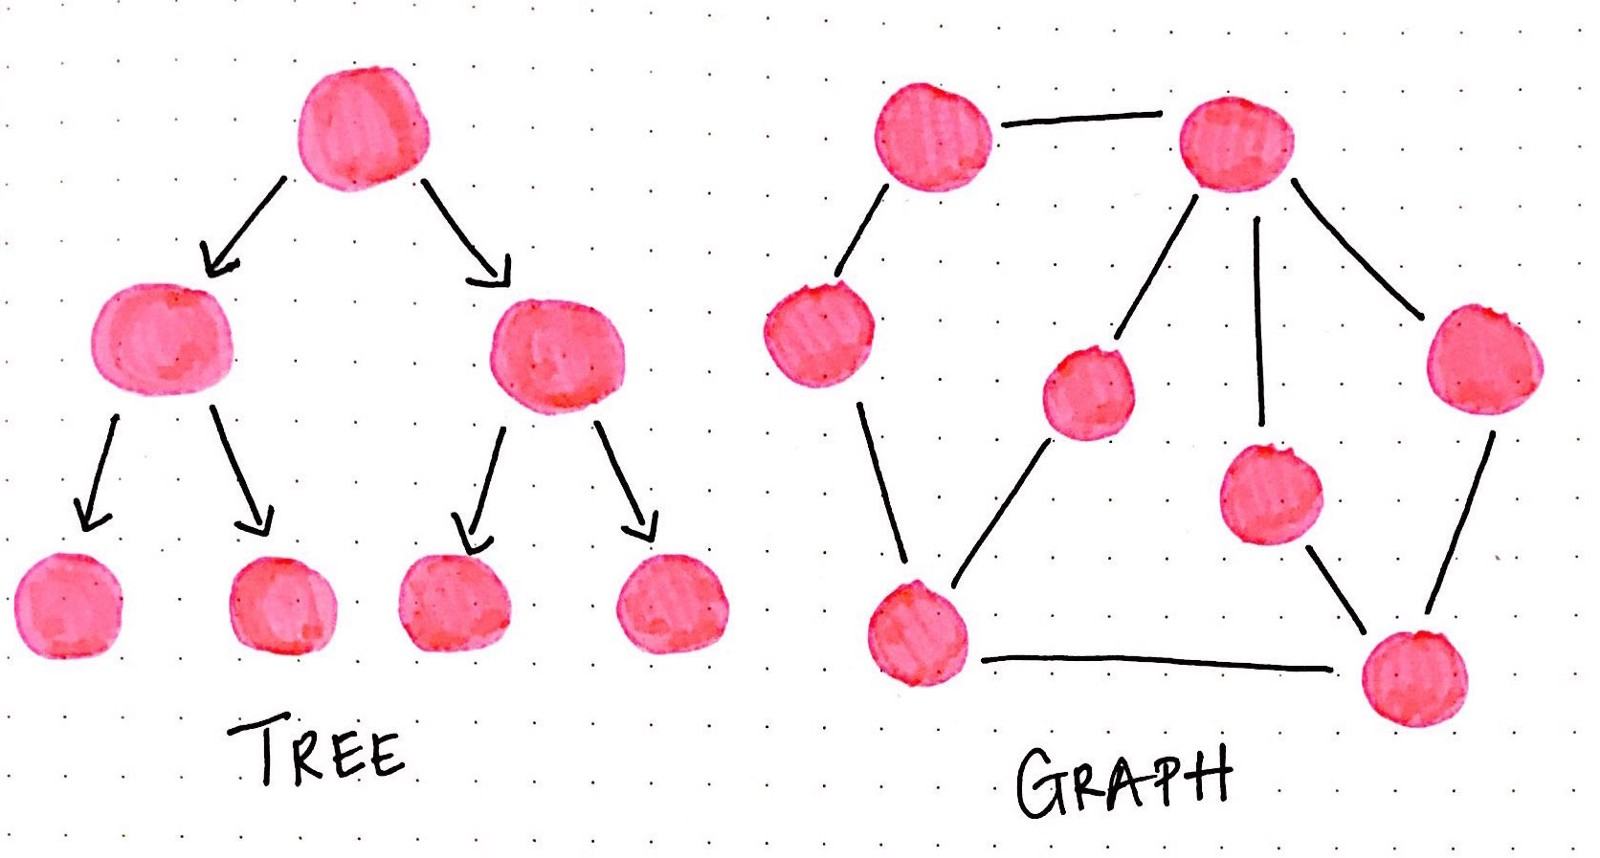
\includegraphics[scale=.15]{trees-graphs.jpeg}

We will utilize this model of our tree to develop out and algorithm identifying the magnitude and location of both branch flows that contribute to through fall, and branch flows that contribute to stem flow. This technique continues as follows:


\begin{itemize}
  \item Assign the following attributes to each node with null value: FlowId, FlowType, isDripPoint, isDividePoint
  \item Assign the following attributes to each edge with the value of the corrosponding cylinder: length, SurfaceArea, UnitVector, projectedsurfacearea 
  \item Identify all nodes that are present in the trunk (these are nodes that have an order of 0 as per computree) and remove them from the tree
  \item Place the remaining connected components (representing all branches that can possibly contribute to branch flow) in a collection; iterate over this collection.
  \item For each cylinder, identify the end nodes (the nodes representing end points of cylinders with no children) and the root node ( the beginning point of the singular cylinder without a parent
  \item Calculate the shortest path (the only path in fact, from each end node to the root node
  \item for each end node -> root path, step through the graph from end node to root path
  
\end{itemize}

Then we create an array 'flows' that has one row for each 
For each node in a given path, and the edge it immediately connects to:
\begin{itemize}
    \item calculate the angle of the cylinder via the unit vector
    \item Add the length, surface area and angle to a running sum
    \item If the edge is angled downward as traveled towards the trunk along our graph (thus has 'in-flow')
    \begin{itemize}
        \item If the next edge also has 'in flow' and a similar angle to the current edge
        \begin{itemize}
            \item If the next edge also has 'in flow' and a similar angle to the current edge
    
        \end{itemize}
    \end{itemize}
\end{itemize}
    

*****************Lorem ipsum dolor sit amet, consectetur adipiscing elit, sed do eiusmod tempor incididunt ut labore et dolore magna aliqua. Ut enim ad minim veniam, quis nostrud exercitation ullamco laboris nisi ut aliquip ex ea commodo consequat. Duis aute irure dolor in reprehenderit in voluptate velit esse cillum dolore eu fugiat nulla pariatur. Excepteur sint occaecat cupidatat non proident, sunt in culpa qui officia deserunt mollit anim id est laborum.

Lorem ipsum dolor sit amet, consectetur adipiscing elit, sed do eiusmod tempor incididunt ut labore et dolore magna aliqua. Ut enim ad minim veniam, quis nostrud exercitation ullamco laboris nisi ut aliquip ex ea commodo consequat. Duis aute irure dolor in reprehenderit in voluptate velit esse cillum dolore eu fugiat nulla pariatur. Excepteur sint occaecat cupidatat non proident, sunt in culpa qui officia deserunt mollit anim id est laborum.

Lorem ipsum dolor sit amet, consectetur adipiscing elit, sed do eiusmod tempor incididunt ut labore et dolore magna aliqua. Ut enim ad minim veniam, quis nostrud exercitation ullamco laboris nisi ut aliquip ex ea commodo consequat. Duis aute irure dolor in reprehenderit in voluptate velit esse cillum dolore eu fugiat nulla pariatur. Excepteur sint occaecat cupidatat non proident, sunt in culpa qui officia deserunt mollit anim id est laborum.

Lorem ipsum dolor sit amet, consectetur adipiscing elit, sed do eiusmod tempor incididunt ut labore et dolore magna aliqua. Ut enim ad minim veniam, quis nostrud exercitation ullamco laboris nisi ut aliquip ex ea commodo consequat. Duis aute irure dolor in reprehenderit in voluptate velit esse cillum dolore eu fugiat nulla pariatur. Excepteur sint occaecat cupidatat non proident, sunt in culpa qui officia deserunt mollit anim id est laborum.

\subsection{Sample subsection}
Sample text. Sample text. Sample text. Sample text. Sample text. Sample text. 
Sample text. Sample text. Sample text. Sample text. Sample text. Sample text. 

Lorem ipsum dolor sit amet, consectetur adipiscing elit, sed do eiusmod tempor incididunt ut labore et dolore magna aliqua. Ut enim ad minim veniam, quis nostrud exercitation ullamco laboris nisi ut aliquip ex ea commodo consequat. Duis aute irure dolor in reprehenderit in voluptate velit esse cillum dolore eu fugiat nulla pariatur. Excepteur sint occaecat cupidatat non proident, sunt in culpa qui officia deserunt mollit anim id est laborum.

\subsubsection{Sample subsubsection}
Sample text. Sample text. Sample text. Sample text. Sample text. Sample text. 
Sample text. Sample text. Sample text. Sample text. Sample text. Sample text. 


Results are presented in Table~\ref{tab1}.
\begin{table}[!htb]
\caption{Sample table.}\label{tab1}
\begin{tabular}{ccc}
\hline\\[-1.5ex]
AAA & BBB & CCC \\[0.5ex]
\hline\\[-1.5ex]
1.0 & 2.0 & 3.0\\[0.5ex]
1.0 & 2.0 & 3.0\\[0.5ex]
\hline
\end{tabular}
\end{table}


\bibliography{sample}

\end{document}
